\section{Results: combined frictions}
\label{sec:results-factorial}

\subsection{Design recap and benchmark predictions}
\label{sec:factorial-design-recap}

The factorial described in Section~\ref{sec:methodology-combined} crosses all three frictions at two levels each:
\begin{align*}
    L \in \{0,\, 2\}, \qquad
    \sigma \in \{0,\, 1\}, \qquad
    T \in \{0,\, 1\}.
\end{align*}
The eight cells $\texttt{F}abc$ ($a,b,c \in \{0,1\}$) span every combination. Each cell was run at three replication sizes ($N\in\{250,500,1000\}$ sessions) to confirm that the interaction pattern is stable to sampling noise.

For each multi-friction cell we compare the observed $\Delta$ against three benchmark predictions:
\begin{description}[leftmargin=2.4em, style=nextline]
    \item[Additive] $\widehat{\Delta}_{\mathrm{add}} \;=\; \max\!\bigl\{0,\; \Delta_{0} - \sum_{i\in\mathcal{F}} \bigl(\Delta_{0} - \Delta_{i}\bigr)\bigr\}$, where $\mathcal{F}$ is the set of frictions ``on'' in the cell, $\Delta_0$ the baseline, and $\Delta_i$ the corresponding single-friction value.
    \item[Multiplicative] $\widehat{\Delta}_{\mathrm{mult}} \;=\; \Delta_{0} \cdot \prod_{i\in\mathcal{F}} \Delta_{i}/\Delta_{0}$.
    \item[Minimum] $\widehat{\Delta}_{\mathrm{min}} \;=\; \min_{i\in\mathcal{F}} \Delta_{i}$ --- the most-destructive single friction wins.
\end{description}
The additive prediction is the naive ``effects add'' benchmark and is clearly wrong at the extremes (sums of $>100\%$ reductions are nonsense), but it is reported for completeness because it is the prediction one would write down without thinking carefully. The multiplicative prediction treats each friction's relative damage to $\Delta$ as an independent dampening factor. The minimum prediction is the prediction one would make if frictions did not interact at all and the strongest one entirely determined the outcome.\todo{Consider also reporting a ``maximum'' prediction (collusion is preserved up to the level of the weakest friction). Symmetric to ``minimum'' in spirit; could be a complementary comparison point.}

\subsection{Cross-validation of the unified implementation}
\label{sec:factorial-crosscheck}

Four cells of the factorial constitute internal cross-validation against the single-friction implementations of Section~\ref{sec:results-singles}, since they correspond to inputs at which the unified learner should reproduce the corresponding single-friction learner exactly:
\begin{itemize}[topsep=0pt, itemsep=2pt]
    \item \texttt{F000} $(0,0,0)$: should reproduce the baseline.
    \item \texttt{F100} $(2,0,0)$: should reproduce the latency-only cell at $L=2$.
    \item \texttt{F010} $(0,1,0)$: should reproduce the noise-only cell at $\sigma=1$.
    \item \texttt{F001} $(0,0,1)$: should reproduce the async-only cell at $T=1$.
\end{itemize}

Table~\ref{tab:factorial-crosscheck} compares the four cells of the unified factorial against the corresponding single-friction runs. The factorial cells reproduce the single-friction values to five decimal places, providing strong evidence that the unified learner correctly composes the three frictions.

\begin{table}[H]
\centering
\caption{Cross-validation: unified factorial cells reproduce single-friction results.}
\label{tab:factorial-crosscheck}
\begin{tabular}{lcc}
\toprule
Cell                       & Single-friction $\Delta$ & Factorial $\Delta$ \\
\midrule
\texttt{F000} (baseline)   & $0.84280$ & $0.84280$ \\
\texttt{F100} ($L=2$)      & $0.21490$ & $0.21490$ \\
\texttt{F010} ($\sigma=1$) & $0.49269$ & $0.49269$ \\
\texttt{F001} ($T=1$)      & $0.37833$ & $0.37833$ \\
\bottomrule
\end{tabular}
\end{table}

\subsection{Headline results at \texorpdfstring{$N=1000$}{N=1000}}
\label{sec:factorial-headline}

Table~\ref{tab:factorial-1000} reports all eight cells at the highest replication size ($N=1000$ sessions per cell). Figure~\ref{fig:factorial-forest} renders the same data as a forest plot against the three benchmark predictions. The $N=250$ and $N=500$ replications appear in Section~\ref{sec:factorial-stability}.

\begin{table}[H]
\centering
\caption{$2\times 2\times 2$ factorial at $N=1000$ sessions per cell. SD is the cross-session standard deviation of $\Delta$. $\widehat{\Delta}_{\mathrm{add}}$, $\widehat{\Delta}_{\mathrm{mult}}$ and $\widehat{\Delta}_{\mathrm{min}}$ are the additive, multiplicative and minimum benchmark predictions of Section~\ref{sec:factorial-design-recap}.}
\label{tab:factorial-1000}
\renewcommand{\arraystretch}{1.05}
\begin{tabular}{lcccccc}
\toprule
Cell & $(L,\sigma,T)$ & $\Delta$ (obs.) & SD & $\widehat{\Delta}_{\mathrm{add}}$ & $\widehat{\Delta}_{\mathrm{mult}}$ & $\widehat{\Delta}_{\mathrm{min}}$ \\
\midrule
\texttt{F000} & $(0,0,0)$ & $0.848$ & $0.109$ & ---     & ---     & ---     \\
\texttt{F100} & $(2,0,0)$ & $0.210$ & $0.122$ & ---     & ---     & ---     \\
\texttt{F010} & $(0,1,0)$ & $0.500$ & $0.298$ & ---     & ---     & ---     \\
\texttt{F001} & $(0,0,1)$ & $0.383$ & $0.111$ & ---     & ---     & ---     \\
\midrule
\texttt{F110} & $(2,1,0)$ & $0.059$ & $0.080$ & $0.000$ & $0.124$ & $0.210$ \\
\texttt{F101} & $(2,0,1)$ & $0.346$ & $0.174$ & $0.000$ & $0.094$ & $0.210$ \\
\texttt{F011} & $(0,1,1)$ & $0.280$ & $0.103$ & $0.034$ & $0.226$ & $0.383$ \\
\texttt{F111} & $(2,1,1)$ & $0.537$ & $0.135$ & $0.000$ & $0.056$ & $0.210$ \\
\bottomrule
\end{tabular}
\end{table}

\begin{figure}[H]
\centering
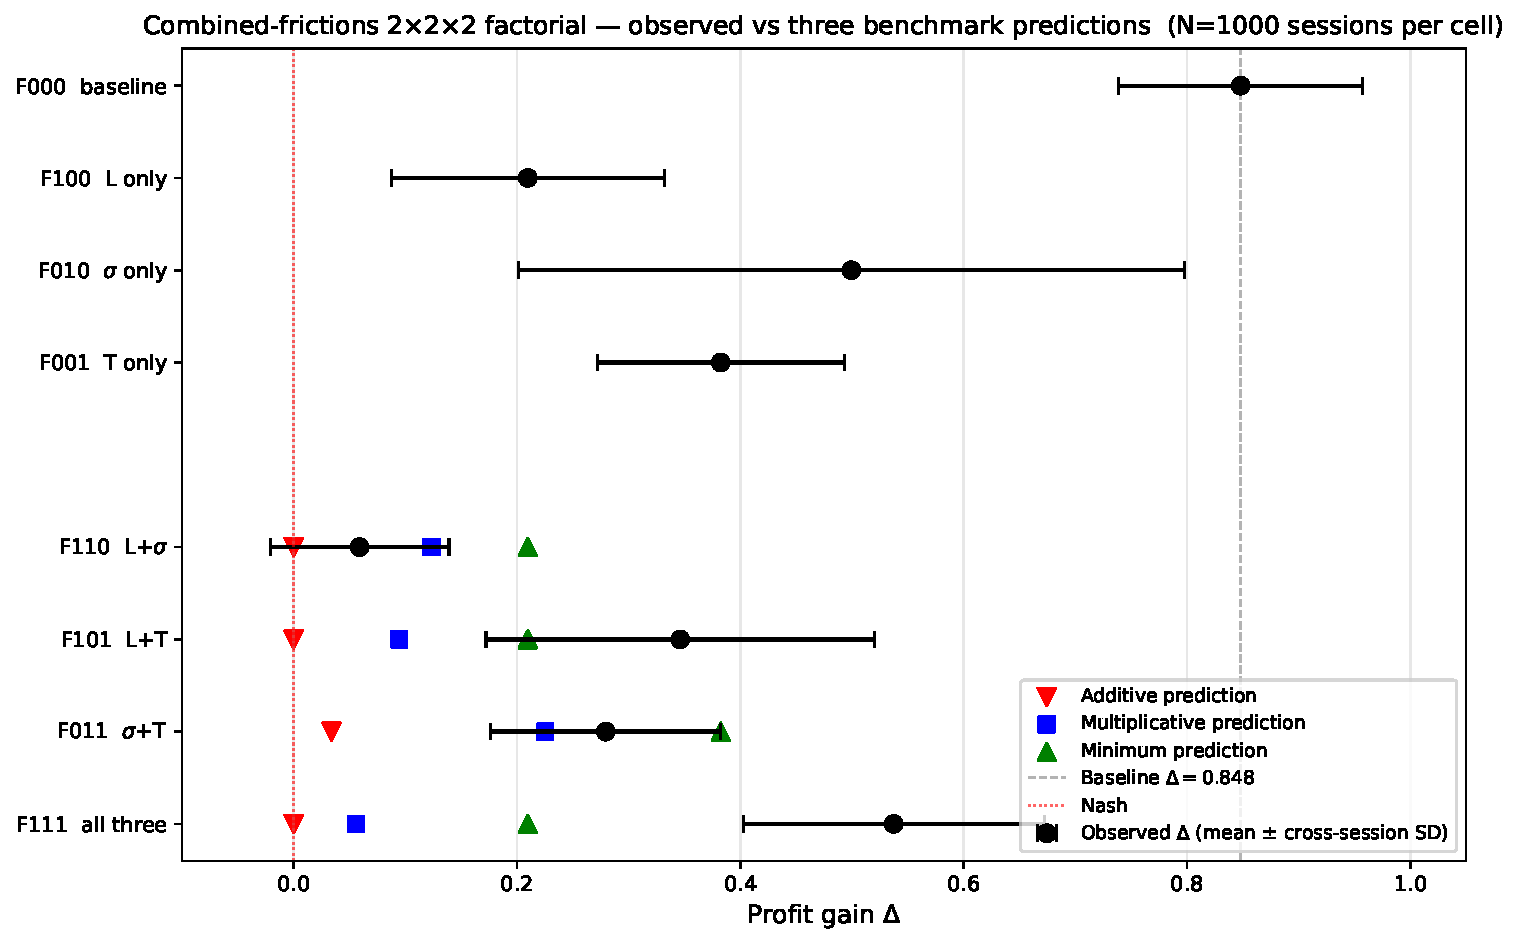
\includegraphics[width=0.95\linewidth]{figures/fig_factorial_forest.pdf}
\caption{Combined-frictions $2\times 2\times 2$ factorial at $N=1000$. Black points: observed $\Delta$; horizontal bars: cross-session SD. Coloured markers: additive (red), multiplicative (blue) and minimum (green) benchmark predictions for each multi-friction cell.}
\label{fig:factorial-forest}
\end{figure}

The four interesting cells are the four below the rule in Table~\ref{tab:factorial-1000}. Each tells a different story.

\subsubsection*{F110 (latency $+$ noise) --- super-multiplicative compounding}
The observed $\Delta = 0.059$ is below the multiplicative prediction of $0.124$ and well below the minimum prediction of $0.210$. Combining moderate latency with moderate noise destroys more of the collusion than either friction's relative effect would suggest if their dampenings were independent. The two frictions act on different dimensions of the rival-side observation --- latency on its time of arrival, noise on its value --- and stacking them produces a signal that is both stale and wrong, which is more disruptive to learning than either error alone.

\subsubsection*{F011 (noise $+$ async) --- approximately multiplicative}
The observed $\Delta = 0.280$ is reasonably close to the multiplicative prediction of $0.226$, though somewhat above it. The closeness is interesting: this is the only multi-friction cell where the multiplicative model is approximately correct.

\subsubsection*{F101 and F111 --- async ``rescues'' collusion}
The two cells with $T=1$ on top of latency (\texttt{F101}, \texttt{F111}) tell the most surprising story. \texttt{F101} ($L=2$, $T=1$) yields $\Delta = 0.346$, \emph{higher} than the latency-only cell \texttt{F100} ($\Delta = 0.210$). Adding asynchrony on top of latency \emph{increases} collusion. The same pattern is even more pronounced in the all-frictions cell \texttt{F111}: $\Delta = 0.537$ is higher than \texttt{F110} ($\Delta = 0.059$, latency $+$ noise alone), and indeed higher than every multi-friction cell that lacks asynchrony.

This is an opposite-sign interaction: asynchrony alone reduces $\Delta$ from $0.848$ to $0.383$, but adding asynchrony on top of latency (or latency-and-noise) increases $\Delta$ relative to those baselines. The mechanism story we tentatively offer is that strict alternation imposes a one-period structural commitment on the moving agent's rival, providing the moving agent with a stable target against which to optimise. When the rival's signal is itself corrupted (by noise) or stale (by latency), this structural commitment partially substitutes for the missing information. The agents can coordinate on the commitment schedule itself rather than on the agent's strategy, which is unobservable through the corrupted signal.\todo{This mechanism story is plausible but speculative. Off-path deviation analysis (sensu \citealp{calvano2023}) would help adjudicate: do the F101 and F111 strategies support genuine punishment, or are they spurious focal-point equilibria? Add this to limitations / future work.}

\subsection{Stability across replication sizes}
\label{sec:factorial-stability}

A natural concern is that the headline pattern --- particularly $\Delta_{\texttt{F111}} > \Delta_{\texttt{F110}}$ and $\Delta_{\texttt{F101}} > \Delta_{\texttt{F100}}$ --- could be sampling noise. Table~\ref{tab:factorial-acrossN} reports all eight cells at $N\in\{250,500,1000\}$.

\begin{table}[H]
\centering
\caption{Factorial $\Delta$ across replication sizes. Movements between columns are within sampling noise; the qualitative pattern is identical at all three $N$.}
\label{tab:factorial-acrossN}
\renewcommand{\arraystretch}{1.05}
\begin{tabular}{lccc}
\toprule
Cell & $\Delta\;(N{=}250)$ & $\Delta\;(N{=}500)$ & $\Delta\;(N{=}1000)$ \\
\midrule
\texttt{F000} & $0.843$ & $0.842$ & $0.848$ \\
\texttt{F100} & $0.215$ & $0.212$ & $0.210$ \\
\texttt{F010} & $0.493$ & $0.496$ & $0.500$ \\
\texttt{F001} & $0.378$ & $0.385$ & $0.383$ \\
\texttt{F110} & $0.063$ & $0.062$ & $0.059$ \\
\texttt{F101} & $0.323$ & $0.343$ & $0.346$ \\
\texttt{F011} & $0.264$ & $0.277$ & $0.280$ \\
\texttt{F111} & $0.551$ & $0.539$ & $0.537$ \\
\bottomrule
\end{tabular}
\end{table}

\begin{figure}[H]
\centering
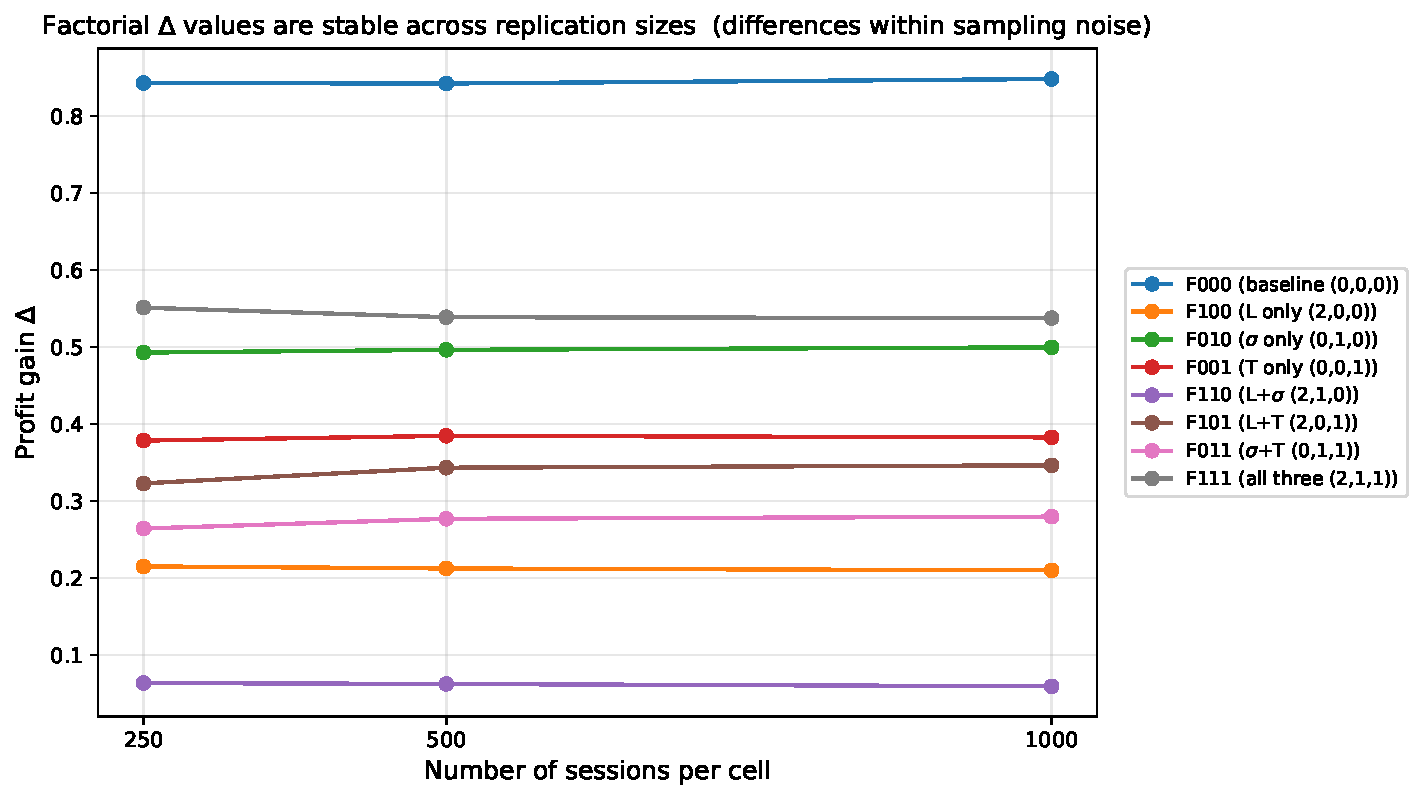
\includegraphics[width=0.95\linewidth]{figures/fig_factorial_acrossN.pdf}
\caption{Factorial $\Delta$ values at $N\in\{250,500,1000\}$ for all eight cells. The observed pattern is qualitatively identical across replication sizes, with cell-level movements between $N$'s typically below $0.02$.}
\label{fig:factorial-acrossN}
\end{figure}

The cell-level $\Delta$ values move by less than $0.025$ between $N=250$ and $N=1000$. The headline interaction patterns --- super-multiplicative compounding of $L$ and $\sigma$, async rescuing collusion in \texttt{F101} and \texttt{F111} --- are visually identical at all three replication sizes. The standard error of the mean across sessions, $\mathrm{SD}/\sqrt{N}$, is approximately $0.004$ at $N=1000$ on the headline cells, well below any of the inter-cell differences that drive the interpretation. We therefore consider the interaction pattern robust to sampling noise.

\subsection{Summary of factorial findings}
\label{sec:factorial-summary}

Three findings emerge that survive replication and that we carry into the discussion:
\begin{enumerate}[topsep=2pt, itemsep=2pt]
    \item Latency and noise compound \emph{super-multiplicatively}.
    \item Asynchrony, in combination with either latency or noise (or both), \emph{partially restores} collusion that the other frictions would otherwise destroy --- an opposite-sign interaction with respect to the main effect of asynchrony.
    \item No single benchmark prediction (additive, multiplicative, or minimum) describes all four multi-friction cells. The factorial therefore rejects the simplest models of how frictions ought to combine.
\end{enumerate}
